\chapter{Programming Documentation - Platform}
\label{attachments:programming-platform}
This document serves as a programming documentation for the platform.
Covers the mono-repo setup that houses both the client-side React applications and the server-side API services.
This document is intended to guide developers through system setup, project structure, feature integration, and daily tasks.

The first Section \ref{attachments:programming-platform.project-structure} will present the complete structure of the platform, including the description of the components.
Then, in the Section \ref{attachments:programming-platform.coding-convention} we will go through and describe the coding conventions that are recommended to follow when working on the platform.
The third \ref{attachments:programming-platform.technical-design} Section will provide brief overview of the technical design of the platform.
Next, the fourth Section \ref{attachments:programming-platform.backend} will introduce the backend of the platform, including segmentation of project parts and technical details such as authorization, authentication, data filtering and general communication with shipping carriers.
In the fifth Section \ref{attachments:programming-platform.frontend} we will present frontends with several decision and key elements influencing the project.
Next, in the Section \ref{attachments:programming-platform.integrating}, we will delve into a way how to integrate new features, such as shipping carriers, but also essential things such as adding new environment variable.
In the Section \ref{attachments:programming-platform.infrastructure} several important infrastructure points from programmers perspective will be presented.
And lastly, in the Section \ref{attachments:programming-platform.docs}, some information regarding user documentation will be provided. 


\section{Project structure}
\label{attachments:programming-platform.project-structure}
The platform uses a monorepo architecture to house both frontend and backend components under a single repository.
This approach simplifies dependency management, and enhances re-usability across the codebase.
The monorepo includes:
\begin{itemize}
    \item \textbf{Clients:} Containing all React frontend applications and dashboard user documentation.
    \item \textbf{Services:} Housing the API backend service.
    \item \textbf{Infrastructure:} Definitions and configurations of the deployment and operational infrastructure.
\end{itemize}

\subsubsection{Clients}
The clients section currently contains all three frontend projects:
\dirtree{%
.1 clients.
.2 docs/.
.2 tracking/.
.2 web/.
}

Here, the \texttt{docs} project is a Doctosaurus user documentation. The \texttt{tracking} and \texttt{web} are React applications, first for parcel recipients and second is dashboard for the actual users of the platform.

\subsubsection{Services}
The Services folder contains only one service, \texttt{api} - Koa backend.
\dirtree{%
.1 services.
.2 api/.
}

\subsubsection{Infrastructure}
The Infrastructure folder contains all the necessary setups for the deployment in \ac{AWS}.
\dirtree{%
.1 infrastructure.
.2 apps/.
.2 constructs/.
.2 stacks/.
}
The \texttt{apps} folder contains the deployment entry point file. It is where all \texttt{stacks} are initialised for the requested environment.
In the \texttt{constructs} we can find several AWS Constructs.
These are classes inherited from \texttt{Construct} from package \texttt{constructs} defining so-called "piece of system state".
In our case, the constructs are used to define the database, the gateways, the policies, and the S3 bucket for the user uploaded assets.
And lastly, \texttt{stacks} is where the actual services are defined.
Using data from \texttt{aws-cdk-lib.Stack}, they define actual CloudFormation stacks.
Having said that, there is a stack for api, dashboard (webapp), tracking page, documentation, and a specific stack for certificates.



\subsection{Package management}
The platform uses Yarn as its package manager.
Yarn Workspaces are utilised to link together frontend and backend packages, allowing share dependencies installed at the root level optimising disk usage and installation process.
The dependencies for individual projects within the monorepo are declared in their \texttt{package.json} files.
The root \texttt{package.json} includes scripts and dependencies applied throughout the repository.

\section{Coding convention}
\label{attachments:programming-platform.coding-convention}
\subsection{Style guide}
It is recommended to adhere to the Airbnb JavaScript and React style guide for both backend and frontend code.
Including consistent use of modern Java\-Script syntax and readable formatting.
Please use linter regularly, each workspace within the repository contains \texttt{eslint} which can be run by \texttt{yarn check:lint}.
\subsection{File naming}
It is recommended to use \texttt{kebaba-case} for file names.
However, in the React frontend codebase, \texttt{PascalCase} is usually used except for the layout components.

\section{Technical design}
\label{attachments:programming-platform.technical-design}

% brief intro into the technical design with diagrams from chap4.
The platform overview can be seen on Figure \ref{imgdocs:programming-platform.technical-design}.

\begin{figure}[H]\centering
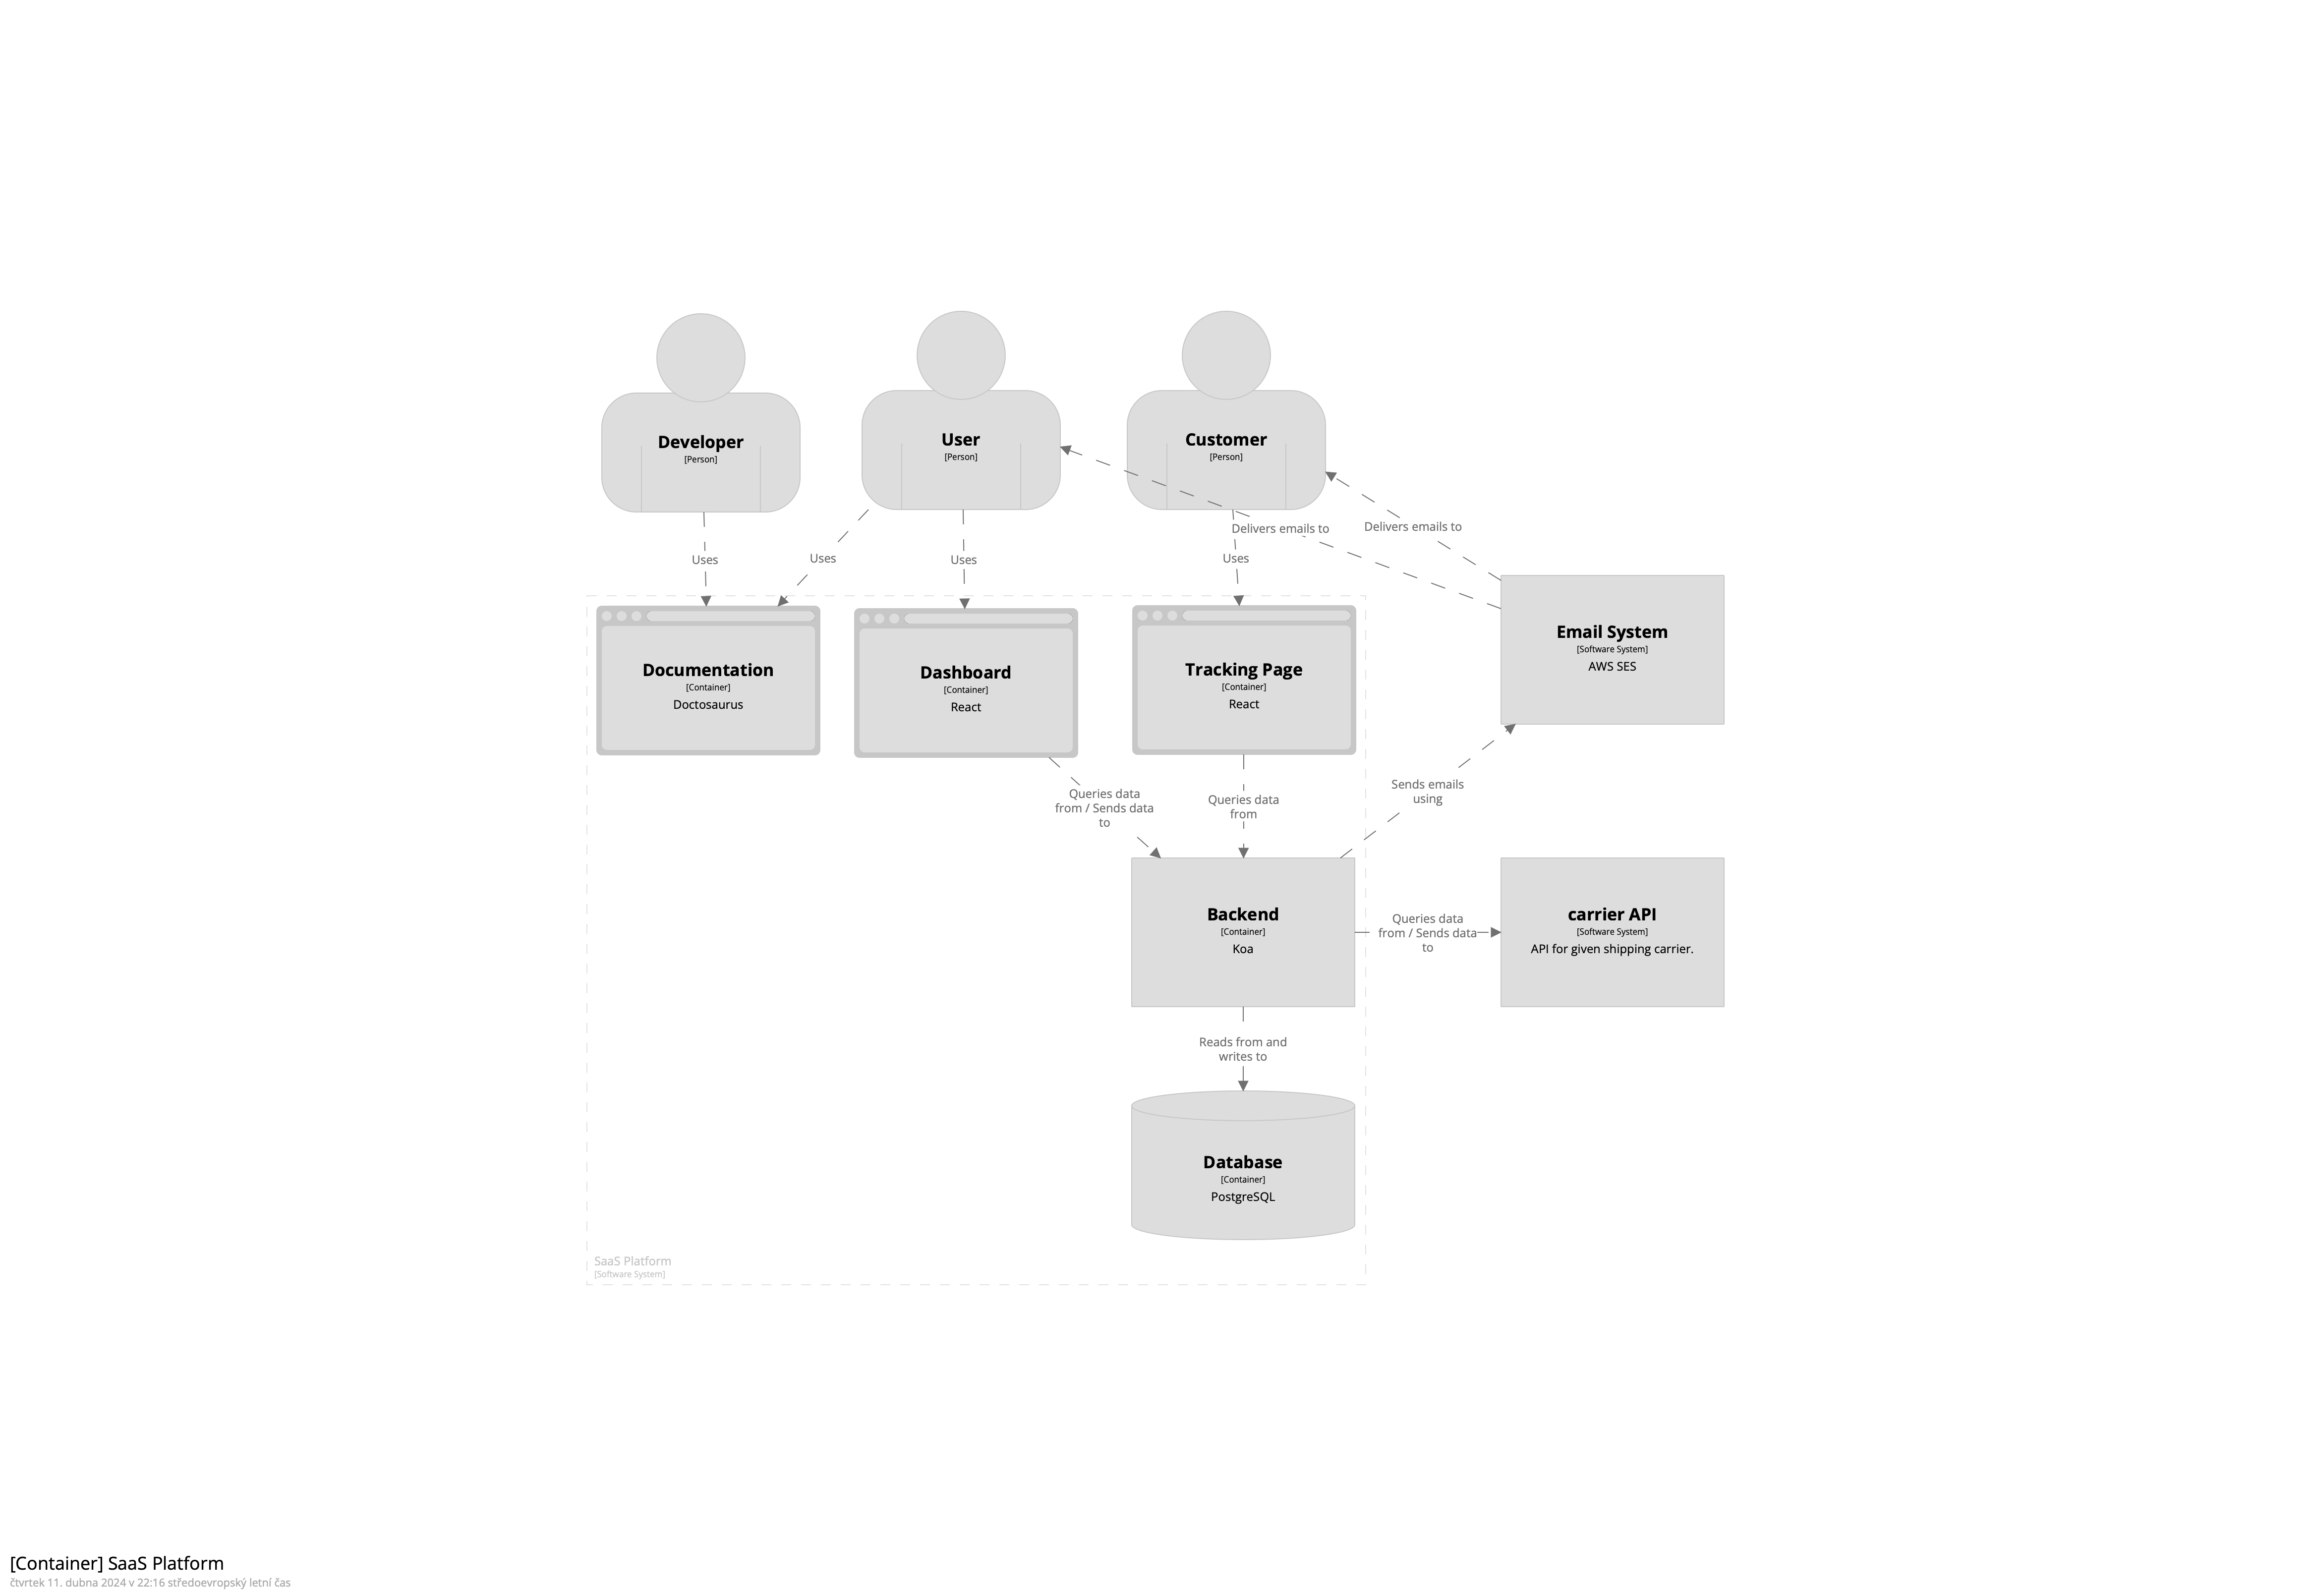
\includegraphics[width=140mm]{img/chap04/fig_architecture.png}
\caption{C4 overview of the architecture}
\label{imgdocs:programming-platform.technical-design}
\end{figure}


\section{Backend}
\label{attachments:programming-platform.backend}
The backend service serves as the central centre for processing all logistic operations, interfacing with external carriers, and managing user interactions through the API. 
Developed using Node.js and the Koa framework, it provides scalable server-side logic.
The project is in the \texttt{services/api/} directory.
The platform is built around several key components in the following order:
\begin{enumerate}
    \item \textbf{Router:} Is main entry of the API where all endpoints are defined.
    \item \textbf{Middlewares:} Are chain-able methods initiated at the beginning of endpoint request or at the end to modify response. They handle authorization, authentication, schema validation, parsing pagination, or filter requests.
    \item \textbf{Actions:} Actions present the "called" method of the endpoint after request middleware.
    \item \textbf{Entities:} Objects stored in the connected database.
    \item \textbf{Services:} Manage the database interactions.
    \item \textbf{Modules:} Defined carrier integrations with unified interface.
\end{enumerate}

The backend elevates the dependency injection container using Microsoft library \texttt{tsyringe}.


\subsection{Database connection}
The database connection reference is stored as a singleton variable at the Lambda handler entry-point (\path{src/lambda-handlers/api.ts}).
This should ensure that no more connections than one are initiated, hence minimising the database load and user connections.

\subsection{Database schema}
Due to the complexity of the database schema, it will be described in following sections:
\begin{itemize}
    \item Projects
    \item Users
    \item Shipments
\end{itemize}

\subsubsection{Projects}
Projects are the main building block of the platform.
They are used as the point of differentiation of data between tenants.
However, each tenant can have access to or own multiple projects (based on their plan).
For the database diagram, refer to Figure \ref{imgdocs:db-schema-projects}.
The project includes a reference to its owner, as well as a name and renewable API key. 
Multiple users can have access to the project and users can be invited into the project.
Each project can contain individual settings of the shipping carrier API (\texttt{project\_shippingcarrier}) and multiple sellers (\texttt{project\_sellers}).
Furthermore, the project contains its global shipper (\texttt{shipper}) reference meant for each shipment in the table.

\begin{figure}[H]\centering
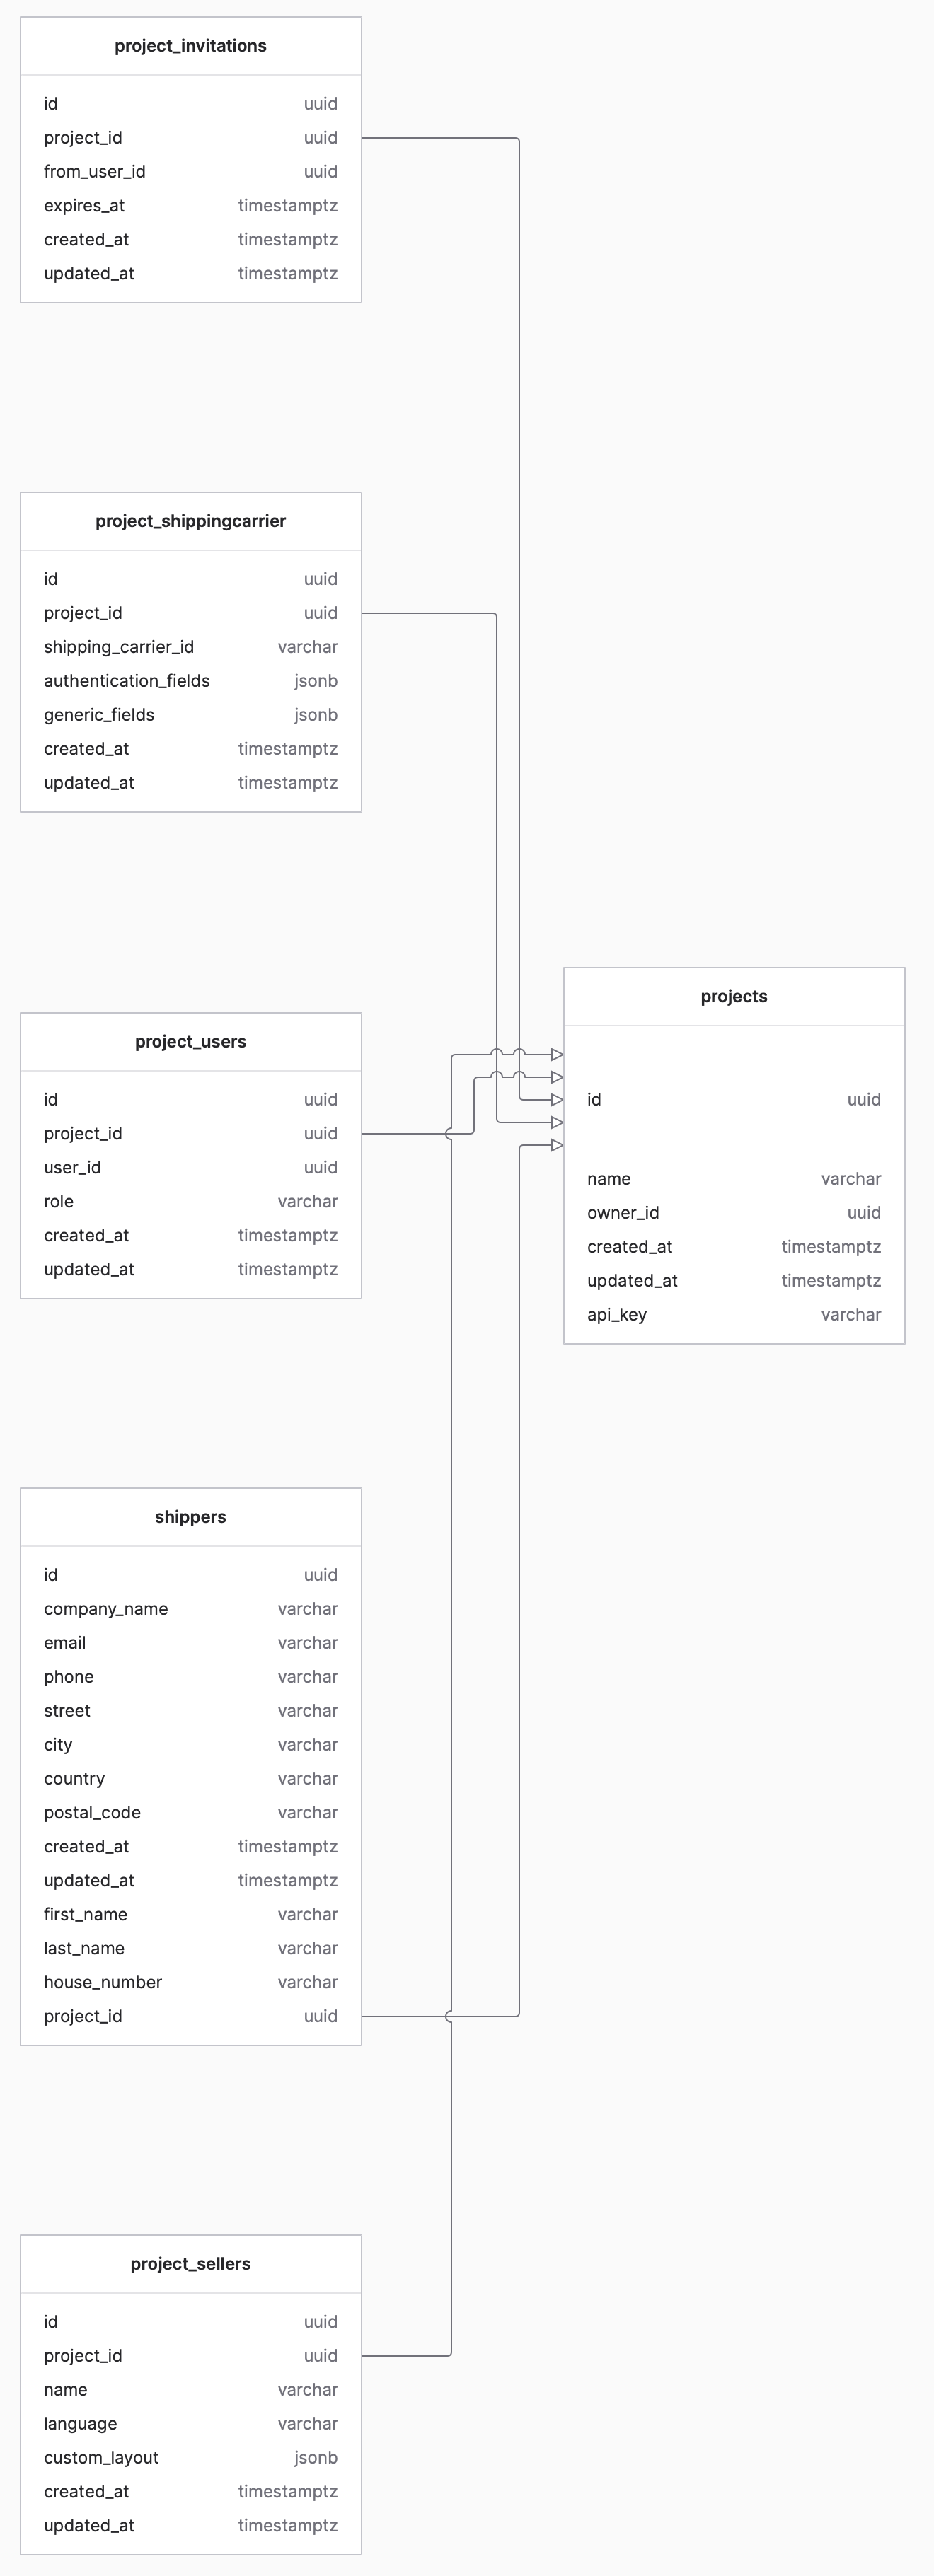
\includegraphics[width=80mm]{img/docs/fig_db_schema_projects.png}
\caption{Database schema diagram of \texttt{Projects} related tables}
\label{imgdocs:db-schema-projects}
\end{figure}

\subsubsection{Users}
The user is an object authenticated and authorised with each request.
For the database diagram, please refer to Figure \ref{imgdocs:db-schema-users}.
If a user owns a project, they have to have a plan defined.

\begin{figure}[H]\centering
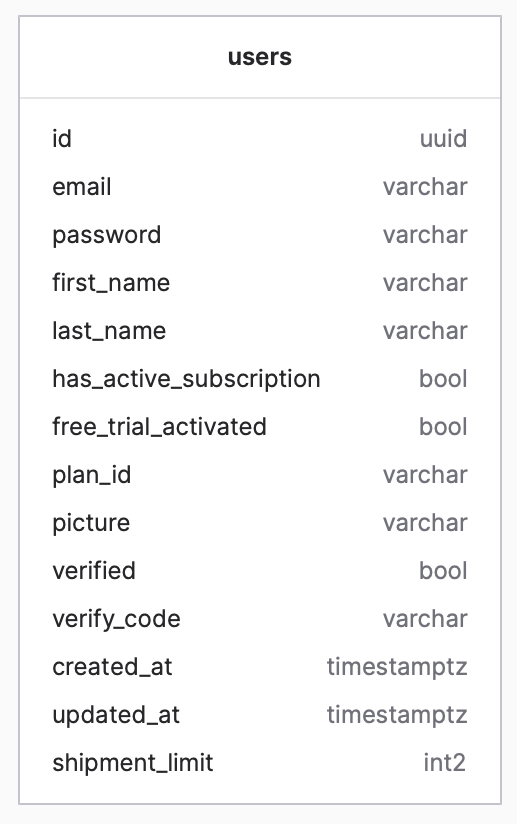
\includegraphics[width=80mm]{img/docs/fig_db_schema_users.png}
\caption{Database schema diagram of \texttt{Users} related tables}
\label{imgdocs:db-schema-users}
\end{figure}

\subsubsection{Shipments}
The shipment is the object with which the user comes into contact the most and also the most important part from a business perspective.
For the database diagram, please refer to Figure \ref{imgdocs:db-schema-shipments}.
Shipment is a complex object constructed from:
\begin{itemize}
    \item \textbf{Parcels:} Representing the actual shipped box with a label and tracking number. Shipment can have multiple parcels.
    \begin{itemize}
        \item \textbf{Parcel status:} Status of each parcel with metadata provided by carrier.
        \begin{itemize}
            \item \textbf{Parcel status type:} A unified type of parcel status with user visible translated textual data. It can take the following values:
            \begin{itemize}
                \item \texttt{EXCEPTION}
                \item \texttt{DATA\_SENT}
                \item \texttt{ACCEPTED\_BY\_CARRIER}
                \item \texttt{HANDED\_OVER}
                \item \texttt{IN\_TRANSIT}
                \item \texttt{OUT\_FOR\_DELIVERY}
                \item \texttt{STORED\_FOR\_PICKUP}
                \item \texttt{PICKED\_UP}
                \item \texttt{DELIVERED}
                \item \texttt{DELIVERY\_FAILED}
                \item \texttt{RETURNED}
                \item \texttt{CANCELED}
            \end{itemize}
        \end{itemize}
    \end{itemize}
    \item \textbf{Shipper:} Universal shipper of the project.
    \item \textbf{Recipient:} The recipient sent to the carrier with the address or pickup point and contact information.
    \item \textbf{Customs, commodities:} For a customs clearance, the user needs to provide information about the parcel.
    \item \textbf{Insurance, payment:} To define a insurance value with currency, as well as payment type and amount.
\end{itemize}

\begin{figure}[H]\centering
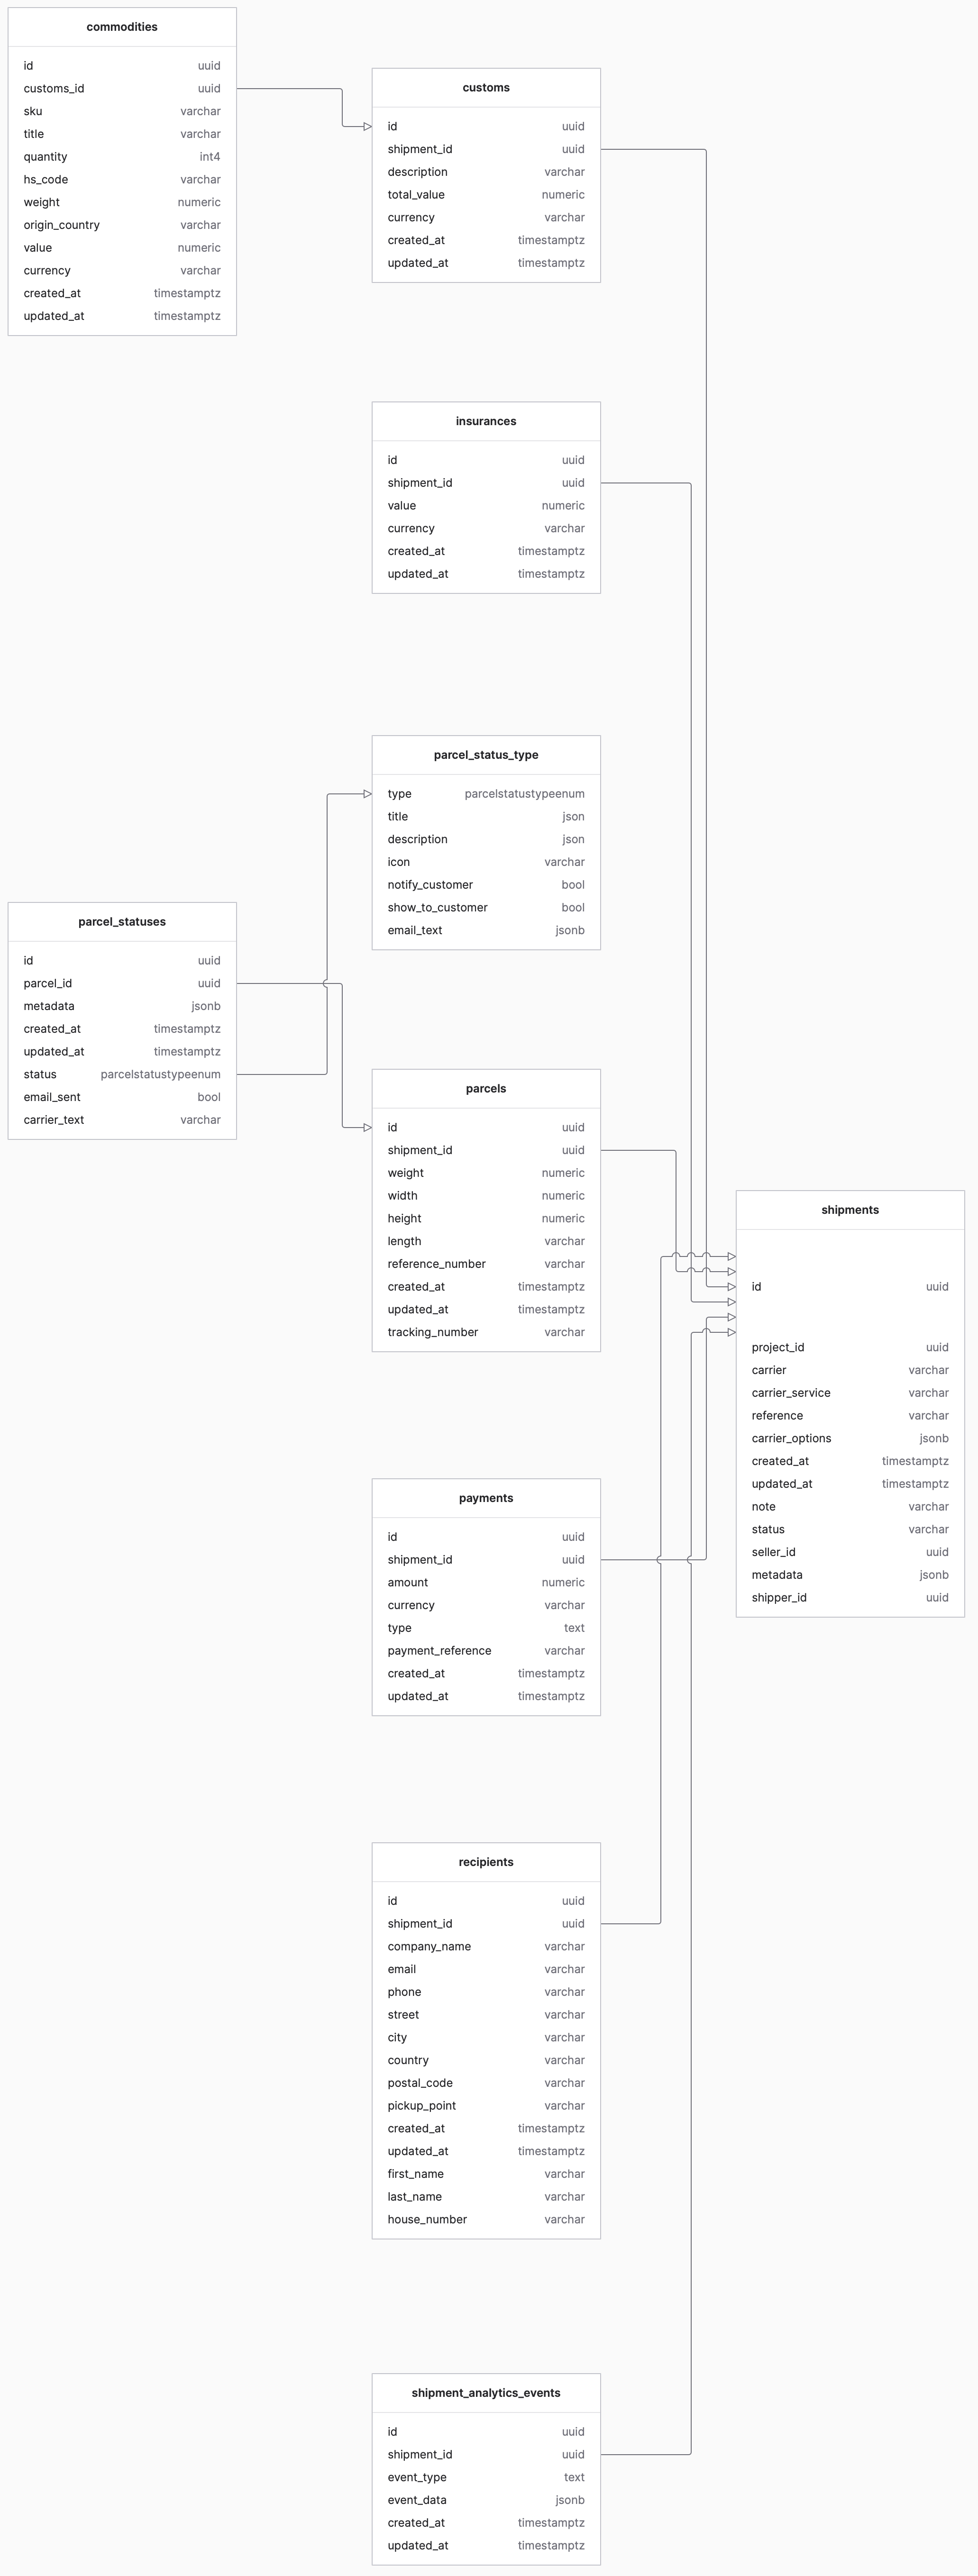
\includegraphics[width=90mm]{img/docs/fig_db_schema_shipments.png}
\caption{Database schema diagram of \texttt{Shipments} related tables}
\label{imgdocs:db-schema-shipments}
\end{figure}
\subsection{Endpoints}
The backend is structured as an API utilising REST principles.
Each endpoint corresponds to a specific function within the platform, allowing \ac{CRUD} operations on resources such as shipments, users, projects, and operations calling carrier APIs. 
All endpoints with related middlewares and actions are defined in \texttt{router.ts}.

\subsection{Authentication and authorisation}
User authentication and authorization is implemented with respect to the best practices of Koa as a middleware.
With this convenient approach, we can "decorate" each route of the API with \texttt{authenticationMiddleware} and, if needed, \texttt{authorizationMiddleware} handling the crucial logic of retrieving user credentials, verifying them and passing them into the \texttt{tsyringe} container for other middlewares, actions or services to utilise the user object.

\subsubsection{Authentication flow}
The authentication is based on token authentication.
\begin{enumerate}
    \item \textbf{Login request:} Users submit their credentials via \path{/authentication/signin}
    \item \textbf{Credential verification:} Credentials are verified against the database entries using hashed passwords.
    \item \textbf{Token generation:} Upon successful authentication, an access and refresh \ac{JWT} is generated and returned to the user.
\end{enumerate}

\subsubsection{Session management}
\begin{itemize}
    \item \textbf{Token storage:} \ac{JWT}s are stored client-side and included in the HTTP authorization header (with \texttt{Bearer} prefix) for requests.
    \item \textbf{Token expiry and refresh mechanism:} Tokens have finite lifetime, after which user must either refresh the token or re-authenticate.
\end{itemize}

\subsubsection{Authorization}
Authorisation is solely based on an authenticated user. 
Each user can have a single role, being either:
\begin{itemize}
    \item Owner
    \item Admin
    \item Member
\end{itemize}

\subsection{Request body validation}
Validating request body on backend is a necessity.
Improve the integrity of the data and the security of the entire system.
For this task, a \gls{joi} library was chosen.
It allows us to simply describe the schema of request body and validate against it.

For an endpoint requiring request body validation it is necessary to define the schema.
For a larger schema, we recommend that you define it in separate file from the file containing the action. 
Then the schema is utilized in the \texttt{schemaValidationMiddleware}.

For example, a schema describing request body where either a list of shipment references or objects containing tracking numbers with carrier name is provided, will look like this:

\begin{lstlisting}[language=JavaScript,caption={Joi schema example}]
import Joi, { Schema } from 'joi';

const schema: Schema = Joi.object({
  shipments: Joi.array().items({
    reference: Joi.string().required(),
  }),
  trackingIds: Joi.object().pattern(
    Joi.string(), // Key as string (carrier name)
    Joi.array().items(Joi.string()) // Value as array of strings
  ),
}).xor('shipments', 'trackingIds'); // Ensure either shipments or trackingIds is provided, but not both
\end{lstlisting}

In order to comply with the DRY principle, \texttt{Joi} schemas are also used to generate OpenAPI specification for the public API.
Each public API should export \texttt{specification} object which, if exists, should contain the \texttt{Joi} schema converted to \texttt{swagger} format using \texttt{joiToSwagger} method.

\subsection{Public API}
So-called "public" methods rely strictly on \texttt{publicApiMiddleware}.
This middleware controls provided \texttt{key} in request headers and attempts to resolve a project related to that value. 
Public API methods are prefixed with \texttt{v1} in the path, and it is necessary to always document them.
Thanks to that we can differentiate whether the request is coming from the user interface or external integration.
This is especially useful when working with shipments.
The shipment alteration uses the UI-first approach, meaning that all shipments created or modified within the user interface cannot be modified through the API.
This is because the integration will usually be done as a periodic data sender which will repeatedly send shipment data until they are marked as "SENT". 
Hence, overwriting user's change which we do not want.


\subsection{OpenAPI schema generation}
After touching on both the topics of request schema description and public API methods, it is a good time to describe the generation of the OpenAPI specification and a Swagger UI. 
The initialisation of an instance of the \texttt{OpenAPI} class is carried out while setting up the server in the Lambda handler.
Each public API endpoint must be registered in the \texttt{OpenAPI} class constructor using the \texttt{registerSpec} function with parameters of the endpoint path and its specification. 
Since the \texttt{OpenAPI} class gets the reference to the Koa router instance as a parameter, we also define the routes \texttt{/openapi.json} and \texttt{/docs} routes.
The Swagger UI is exported from \texttt{openapiUI} method containing the actual Swagger UI HTML with our OpenAPI specification retrieved from \texttt{/openapi.json}.


\subsection{Data filtering}
% describe filtering middleware
Backend handles and provides a lot of data, for this reason it is necessary to provide convenience of data filtering while using the REST API methods provided by backend.
For this purpose \texttt{filterParsingMiddleware} was defined.
This middleware handles the task of parsing query parameters which serve for data filtering.
This filtering syntax is built around this parameter format: \path{?filter=[{FIELD}|{OPERATOR}]={VALUE}}
\\ Where: 
\begin{itemize}
    \item \texttt{FIELD} can be arbitrary field from the response
    \item \texttt{OPERATOR} can be of two types - unary operator or multi-value operator :
    \begin{itemize}
        \item \textbf{Unary:}
        \begin{itemize}
            \item \texttt{EQUALS}
            \item \texttt{CONTAINS}
            \item \texttt{STARTS\_WITH}
            \item \texttt{ENDS\_WITH}
        \end{itemize}
        \item \textbf{Multi-value:}
        \begin{itemize}
            \item \texttt{IN} 
            \item \texttt{BETWEEN}
        \end{itemize}
    \end{itemize}
    \item \texttt{VALUE} can be either a single value when paired with unary operator, or multiple values separated by comma, if multi-value operator is used.
\end{itemize}

These filters are parsed and stored as an array of objects in format \texttt{\{[FIELD]: \{VALUE, OPERATOR\}\}} in the Koa context as the \texttt{filters}.
From this object a database query is then constructed in a service method to which is the object passed as a parameter.

\subsection{Data pagination}
% describe pagination middleware
Handling pagination on backend is essential task with a growing dataset.
For this purpose, \texttt{paginationMiddleware} with supportive types and methods such as \texttt{responsePagination}.
This ensures a unified format of query parameters for both \texttt{page} and \texttt{pageSize} parameters, as well as a response format utilising few of the RESTful principles that return the paginated data set with links to retrieve other data.
The response format is:
\begin{lstlisting}[language=JavaScript,caption={Response pagination type}]
type ResponsePagination = {
  page: number;
  pageSize: number;
  offset: number;
  dataLength: number;
  total: number;
  links: {
    first: string;
    previous: string | null;
    next: string | null;
    last: string;
  };
};
\end{lstlisting}

\subsection{Carrier communication}
% unified set of methods, shipments are groupped into groups by carriers and then resolved separately (by each carrier module)
Integration of shipping carrier APIs is build around abstraction, trying to unify carriers as much as possible to provide seamless user experience without caring about specific details related to each carrier.
All carrier implementations are stored in \path{src/modules/carrier} where each carrier implementation inherits from \texttt{AbstractCarrierModule}.
This abstract class requires from each implementation to contain several public methods which are then used for sending the data, generating files such as labels and waybills, as well as updating or retrieving parcel statuses.

Each carrier is then registered in a dedicated service \texttt{carrier-service} supporting the logic of hiding the details from user experience and, hence, ideally, treating every carrier, from user perspective, as if it was just one.

However, given the fact that each carrier treats their API development differently, there are always some specifics that we cannot fully hide. 
They will be described in the following section.

\subsubsection{Packeta}
% nothing weird, everything has straight forward implementation
Let us start relatively lightly. 
The Packeta API generally does not contain any special features, and the function structure more or less copies the functions in the abstract class.
However, what needed to be modified is the inability to send multiple parcels in a single shipment.
This was done by breaking the shipment into several requests.
This brings us to the next and final point; unfortunately, Packeta does not allow batch shipping of shipments and everything is sent one at a time.
This means a rather lengthy sending of a large amount of data, but due to the relatively fast response time, this does not limit us to the maximum timeout of Lambda functions.

\subsubsection{Česká Pošta}
% async data transfer used for shipping the parcels, parcels has to be picked up using different method, the pickup link is stored in shipment metadata
For the integration with Česká Pošta, our approach leverages asynchronous data transfer techniques to manage parcel shipping. 
Unlike synchronous operations, parcels are not immediately confirmed upon dispatch. Instead, the pickup details are stored within the shipment metadata and must be retrieved through a separate mechanism.
This integration utilises something like a "step function" approach in the Lambda architecture, which allows for asynchronous processing of shipments. This method is particularly advantageous for handling operations that do not provide immediate results, such as waiting for pickup confirmations or processing delayed status updates.
The response retrieved from the request method is stored in the database queue, which is then picked up by separate "pick-up" function retrieving the final response.
% statuses returned from CeskaPosta currently have only date field and not time field. 
% several statuses aren't in the official docs, this might occur again
% method is async so the lamba handler has to be performed as "step function" with storing some metadata

One notable limitation with the Česká Pošta API is that the status updates provided only include the date, not the time. 
This lack of granularity can complicate logistics tracking when precise timing is essential.
Additionally, we have encountered several status codes that are not documented in the official Česká Pošta API documentation.
Such discrepancies suggest that the API might undergo updates or changes that are not immediately reflected in the documentation, posing a challenge to maintaining accurate integration.

\subsubsection{PPL}
% labels are obtain in the process of data transfer, so they are stored as shipment metadata to be picked up anytime within 20 days from transfer
The integration with PPL similarly employs an asynchronous approach to data handling, much like the implementation for Česká Pošta.
 An essential feature of the PPL integration is the handling of shipping labels. 
 Labels are generated at the PPL API side during the data transfer process and are crucial for the physical shipping of parcels. 
 To accommodate the needs of users who may not immediately retrieve these labels, they are stored as an URL reference the shipment metadata and can be accessed at any point within 20 days after the data transfer. 
 This solution ensures that labels are available whenever needed during the period.
 The only downside is that the labels are returned one by one from the PPL.
 So when requesting labels from multiple parcels, it is necessary to obtain each label separately as a JPEG and then construct a single PDF with 4 labels per page using \gls{pdf-lib}.
 The method responsible for this operation is \texttt{\_mergeLabels} defined in \texttt{pplModule}.

\subsection{Generating PDF waybills}
% generating waybills is neccessary feature for every shiper in order to have paper in hand if something weird happens.
% for Packeta, the waybill contains generated barcode which is loaded by the carrier for faster parcel pickup
% it is generated using `import pdf from 'pdfjs'` library as an A4 PDF with custom OpenSans font
Generating PDF waybills meant as a list of shipped parcels with courier's signature is a necessary feature for any shipping operation, providing a document that can serve as a reliable backup in case of discrepancies or issues during the shipping process.
Waybills are generated as A4-sized PDFs using the \gls{pdfjs} library.
The process of generating these documents is designed to be flexible and to accommodate various needs and specifications required by different carriers and regulations. 
Specifically for Packeta, the waybills include a uniquely generated barcode from the Packeta API. 
This barcode facilitates a faster and more efficient parcel pickup process, as the carrier scans it to verify and process the shipment. 
The inclusion of a barcode streamlines the logistics chain, minimising errors and speeding up the time spent in the warehouse.

\section{Frontends}
\label{attachments:programming-platform.frontend}
There are currently three different frontends of two types in the platform.
The first is the user documentation generated by Doctosaurus.
It is located in the \path{clients/docs} folder and contains two language versions, Czech and English.
We will not go into the documentation any further since it follows the official documentation of Doctosaurus.

Let us take a look at the second type of frontend - React.
The platform contains two React frontends - \path{clients/web} serving dashboard and \path{clients/tracking} for displaying tracking information to the recipient.
In this section, we will describe only the React frontends.

\subsection{Overview}
Both React frontends are of similar structure and conventions respecting the typical React project structure with \path{src} directory.
Both projects use functional components with hooks for data fetching and processing.

\subsection{State management}
Elevating Context API principles: passing data through components is done mostly using providers defined within the \path{src/providers} folder. 
This enables to toggle the loading mode, as well as to manage currently selected project in order to differentiate tenants.

\subsection{Routing}
Routing is achieved using \texttt{react-router-dom} package where every protected project route is defined by the project ID in the path. 
Each of these protected paths is wrapped in the \texttt{AuthenticatedRoute} component that controls the validity of the user on every request.

\subsection{Data fetching}
The platform employs a structured approach to data retrieval across its frontend applications, centralizing the logic within custom React hooks to enhance modularity and reusability. 
Each hook is designed to interact with specific backend endpoints, handling various operations such as listing, creating, updating, and deleting projects. 

Data fetching operations utilize the \texttt{useApiActions} custom hook to perform API calls. 
This setup abstracts the complexities of HTTP requests and state management, providing a clear and straightforward API for frontend components to interact with the backend.
The \texttt{executeApiAction} function, central to the mentioned hook, manages the life cycle of API requests. It prepares and sends HTTP requests using the \texttt{ky} library configured with essential hooks for error handling and token refresh logic if needed for protected routes.
Upon completion of an API call, feedback is provided through toast notifications.

\section{Integrating new features}
\label{attachments:programming-platform.integrating}
This section provides guidelines for the integration of new features into the platform. 
Covers the addition of new logistics carriers, the management of environment variables, the handling of frontend metadata, and the implementation of localisation strategies.

\subsection{Adding carriers}
Integrating a new carrier into the platform involves several key steps to ensure a seamless interaction between the platform and the carrier's services. 
This integration typically includes API communication, data parsing, and updating the UI to reflect the new carrier's options.

Steps to integrate a new carrier:
\begin{enumerate}
    \item \textbf{Create carrier type:} Create new value in \texttt{ShippingCarrierId} enumeration in \path{config/types.ts}.
    \item \textbf{Define carrier type:} In the central platform configuration \path{app.config.ts} create a entry in the \texttt{shippingCarriers} array containing the newly defined carrier with all the necessary authentication and generic fields.
    \item \textbf{Defining carrier module:} To create the implementation of the carrier API, it is necessary to create a new file in \path{src/modules/carrier} in the backend that contains a class that implements \texttt{AbstractCarrierModule}.
    \item \textbf{Register the carrier:} In \path{src/services/carrier-service.ts} on backend in the method \texttt{\_createCarrierModule} register the newly created module under the \texttt{ShippingCarrierId} value.
\end{enumerate}
With these steps involved, a new carrier should be integrated into the platform.

\subsection{Database migrations}
A database migration refers to version control of a database schema.
Database migrations produce incremental changes to the schema.
Sometimes, these changes can be reversible. 
Migrations can create a table, add a column, remove it, rename it, or change the type.

All migrations are stored in the \texttt{lib/db/migrations.ts} file within the \texttt{api} directory.
Each migration is inside an array that fully respects the format expected by \gls{knex} library \href{https://knexjs.org/guide/migrations.html#custom-migration-sources}{specified in the \gls{knex} documentation}.
The migration might look like this:
\begin{lstlisting}[language=javascript,caption={Example of a migration from \texttt{migrations.ts}}]
...
{
    name: '16_create_shipment_analytics_events_table',
    up: async (knex: Knex) => {
      await knex.schema.createTable('shipment_analytics_events', (table) => {
        table.uuid('id').defaultTo(knex.raw('uuid_generate_v4()')).primary();
        table
          .uuid('shipmentId')
          .notNullable()
          .index()
          .references('id')
          .inTable('shipments')
          .onUpdate('CASCADE')
          .onDelete('CASCADE');
        table.enum('eventType', ['view', 'click']).notNullable().index().defaultTo('view');
        table.jsonb('eventData').notNullable();
        table.timestamps(true, true);
      });
      return knex;
    },
    down: async (knex: Knex) => {
      await knex.schema.dropTable('shipment_analytics_events');
      return knex;
    },
  },
...
\end{lstlisting}

Running migrations in both local and AWS environment is very straightforward.
We can utilise the following commands which are environment-biased and will run migrations only within the specified environment as long as the database is accessible.
Go to the \texttt{services/api} directory and run:
\begin{itemize}
    \item \texttt{yarn migrate:up:<environment>}: Runs the first unapplied migration in the list.
    \item \texttt{yarn migrate:down:<environment>}: Reverts the last migration applied.
    \item \texttt{yarn migrate:latest:<environment>}: Runs all unapplied migrations.
\end{itemize}

Where the environment can be one of: \texttt{ local | staging | production}.

However, in AWS environments, we recommend leaving migrations for the GitHub action triggered on every push to the \texttt{main} branch.


\subsection{Adding new environment variables}
Adding new environment variable to the whole platform is a very straightforward process.
\begin{enumerate}
    \item Extend the enumeration \texttt{EnvironmentVariable} located in \path{config/types.ts} by the newly added value. If the value should be optional, modify the \texttt{OptionalVariables} type.
    \item In \path{app.config.ts} locate \texttt{environments.environmentVariables} and add a new entry loaded using the \texttt{getEnvVar} method.
    \item For local development, add value to the \texttt{.env} file, for production and staging purposes, add the \texttt{StringParameter} to the \texttt{api-stack}.
\end{enumerate}

\subsection{Passing metadata to frontend}
Metadata provided by the backend are fetched on every load from the frontend.
With this mechanism, we can provide the necessary data to the frontend before every page load.
Bare in mind, that response of this request must be quick - hence, ideally providing just static data. 
The process is straightforward - only modify the \\ \texttt{src/actions/metadata/app-config.ts} action on backend.

\subsection{React Frontend localisation}
Localisation of both React client applications is done using \texttt{i18next} library.  
All translation files are stored within the project in \path{public/locales} folders.
If a new translation key is added, simply run \texttt{yarn generate:locale} within the workspace, and the keys will be generated or modified. 

\section{Infrastructure}
\label{attachments:programming-platform.infrastructure}
This section of the documentation delves into the infrastructure setup that supports the platform's operational and programming decisions. A primary focus is placed on explaining how certain infrastructure choices are closely tied to development practices and user features, such as the direct upload of static assets from the client to the cloud. 

\subsection{Static Asset upload from client}
The platform provides the ability to upload static assets directly from the client to an AWS S3 bucket using presigned URLs, which allows secure, direct browser uploads without exposing server credentials. 
This method optimises the upload process by reducing the server load and network traffic that would otherwise be required if the server had to act as an intermediary.

The backend setup involves a specific route and action handler that generates these presigned URLs. The action, defined in the \texttt{generateSignedUrlAction}, prepares a URL that allows a client to put a file directly into an S3 bucket under a specified path that includes the project ID and the file name.
The \texttt{generateSignedUrlAction} performs the following steps:
\begin{enumerate}
    \item \textbf{Validation:} Ensures required parameters are provided and valid using a Joi schema.
    \item \textbf{Presigned URL Generation:} Uses the AWS SDK's S3RequestPresigner to generate a presigned URL that allows the client to upload a file with public read access. The URL is valid for a short period (e.g., 60 seconds) to enhance security.
    \item \textbf{Response:} Sends the generated URL back to the client, which can be used to upload the file directly to S3
\end{enumerate}

On the frontend, the process to upload a file involves:
\begin{enumerate}
    \item \textbf{Requesting the Presigned URL:} The frontend makes a POST request to the backend to fetch the pre-signed URL, providing the file name as part of the request.
    \item \textbf{File Upload:} Using the received URL, the frontend performs a PUT request using fetch API to upload the file directly to the S3 bucket. The frontend handles upload progress and completion status.
\end{enumerate}

This setup is beneficial for use cases where clients need to upload images or documents related to project sellers, such as banners, logos, or other relevant files. 
The use of AWS S3 ensures scalable and secure storage, while presigned URLs keep AWS credentials safe and provide a method to control access rights on a per-use basis.

\subsection{Sending e-mails}
The functionality for sending emails is defined in \texttt{communication-service.ts} within \texttt{sendEmail} method.
Using \gls{aws-ses} to handle outgoing emails.
This method is responsible for constructing and sending an email through \gls{aws-ses}. It is designed to be flexible, supporting both plain text and HTML email bodies, as well as additional email parameters such as CC, BCC, and reply-to addresses.
The method accepts the following parameters to construct the email:
\begin{itemize}
    \item \textbf{email (string)}: The recipient's email address.
    \item \textbf{subject (string)}: The subject line of the email.
    \item \textbf{textBody (string)}: The plain text body of the email. This is the fallback option for clients that do not support HTML.
    \item \textbf{fromOrganization (string)}: The email address of the sender. By default, this is set to the environment variable \texttt{ORGANIZATION}, which should be configured in the system environment settings.
    \item \textbf{htmlBody (string)}: An optional parameter for the HTML body of the email. If provided, it allows the email to include HTML formatting.
    \item \textbf{replyTo (string)}: An optional parameter specifies the reply-to email address.
    \item \textbf{bccAddresses (array of strings)}: An optional array of BCC (blind carbon copy) addresses for sending the email to additional recipients without disclosing their identities to other recipients.
\end{itemize}
The method initialises a connection to \gls{aws-ses} using \gls{aws-sdk}. 
The \gls{aws-ses} client is configured with the necessary credentials and region information, which are obtained from the environment settings of the platform. Once the client is initialised, the \texttt{sendEmail} method constructs the email parameters into the format required by \gls{aws-ses} and sends the email using the \texttt{SendEmailCommand} from the \gls{aws-sdk}.




\subsection{Time consuming functions}
In the platform architecture, certain operations, such as updating shipment statuses with carriers like Česká Pošta, are time-consuming and require handling that goes beyond the typical execution time limits of AWS Lambda functions. 
To address this, the system uses a two-part method involving request and pickup processes that efficiently manage these operations within Lambda's constraints.
The process is divided into two distinct Lambda functions:
\begin{enumerate}
    \item \textbf{Request Function:} This function is responsible for initiating requests to the carrier's API (e.g., Česká Pošta) for shipment status updates. It handles communication with the external API and then saves the immediate response, which often includes a queue or task ID, in a PostgreSQL database queue. This method allows the function to complete within a short run-time, adhering to Lambda's execution limits.
    \item \textbf{Pickup function:} After the request function stores the task ID in the database, the pickup function takes over. Scheduled or triggered after a predefined interval, this function retrieves the task ID from the queue and makes a subsequent API call to fetch the actual status update. Once the data are received, it processes and integrates the information into the platform's operational flow, updating shipment statuses accordingly.
\end{enumerate}

\subsubsection{Scalability with Step Functions}
With the platform's user base expanding and the volume of shipments growing, the existing method of handling status updates through separate Lambda functions might not scale efficiently. Transitioning the current setup to \gls{step-functions} could offer a more robust solution by orchestrating these operations more dynamically and resiliently.





\section{User documentation}
\label{attachments:programming-platform.docs}
User documentation for the platform's dashboard user interface is created using \gls{doctosaurus}, a dedicated documentation generator that handles the creation of structured and navigable content. 
The documentation files are located within the \texttt{clients/docs} directory of the monorepo, ensuring easy access and version control along with the codebase.
The documentation is available in two languages: Czech and English. 
Any changes to the user interface, modifications to existing functionalities, or the introduction of new features that directly impact how users interact with the platform must be promptly and accurately documented. 
This practice ensures that the documentation remains a reliable and up-to-date resource for end-users, helping them to effectively utilise the dashboard and understand its full range of capabilities. 


